\documentclass[a4paper, 11pt, titlepage]{article}
\usepackage{fancyhdr}
\usepackage{graphicx}
\usepackage{imakeidx}
\usepackage{makeidx}
\usepackage{mathtools}
\usepackage[spanish]{babel}
\usepackage{eurosym}
\usepackage{hyperref}
\usepackage{amssymb}
\usepackage{listings}
\usepackage{xcolor}
\usepackage{subcaption}

\setcounter{secnumdepth}{5}
\setcounter{tocdepth}{5}

\title{{\scshape\Huge Sistemas Operativos Distribuidos \par}}
\author{Francisco Javier Balón Aguilar}

\begin{document}
\maketitle
\renewcommand{\contentsname}{Índice de contenidos} % Nombre dado al ?ndice
\tableofcontents % Genera la tabla de contenidos del ?ndice autom?ticamente
%\newpage

%Lista de figuras 
\listoffigures
%\newpage

%Lista de tablas 
\listoftables
\newpage

\section{Introducción}

    \subsection{Estructura de un sistema distribuido}

        \subsubsection{Funciones de un sistema distribuido}

        \subsubsection{Características de un sistema distribuido}

    \subsection{Tipos de sistemas operativos distribuidos}

\section{Sistemas operativos multiprocesador}

    \subsection{Arquitectura de un sistema operativo multiprocesador}

        Los equipos que cuentan con más de un procesador y que comparten la misma memoria
        se denominan sistemas multiprocesador. En ellos, debe existir un sistema operativo 
        común y central, que controle las operaciones de cada procesador, así como su 
        gestión, coordinación y accesos a memoria.

        Este tipo de sistemas proporcionan una mayor productividad del sistema, ya que 
        pueden realizar un mayor número de tareas en un menor espacio de tiempo, y una 
        mayor velocidad de aplicación, ya que al aumentarse el número de procesadores,
        disminuye el tiempo de espera de un proceso para ser procesado.

        Estos sistemas ofrecen una serie de ventajas:

        \begin{itemize}
            \item \textbf{Rendimiento y potencia de cálculo}.
            \item \textbf{Tolerancia a fallos}.
            \item \textbf{Flexibilidad}.
            \item \textbf{Relación coste/rendimiento}.
        \end{itemize}

        Podemos clasificar los sistemas multiprocesador según el modo de trabajo en:

        \begin{itemize}
            \item \textbf{Procesamiento asimétrico}
            
            El procesamiento asimétrico\footnote{
                El modo de procesamiento asimétrico se originó en 1970 en el Instituto
                 Tecnológico de Massachusetts (M.I.T.). 
            } entre varios ordenadores permite ejecutar procesos 
            de manera independiente separados del procesador que controla y tiene instalado
            el sistema operativo.\footnote{
                A día de hoy este modo de procesamiento no se utiliza casi salvo en 
                aplicaciones muy concretas como puede ser la PS3 de Sony, donde el 
                procesador central tiene sub-procesadores que se encargan de tareas 
                muy específicas.
            }

            Aunque a nivel físico ya no se utilice este diseño de arquitectura, a nivel 
            lógico si que se sigue implantando en sistemas donde cada procesador se encarga
            de una tarea específica, por ejemplo, un procesador puede ser el responsable
            de las operaciones de disco, otro de las operaciones de video, etc. Estos
            sistemas no tienen la flexibilidad de asignación de tareas a los procesadores 
            menos cargados, estando predefinidas por defecto.

            \begin{figure}[htp]
                \centering
                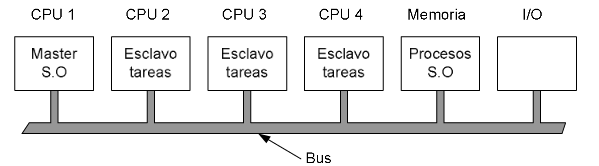
\includegraphics[width=1\textwidth]{resources/multiprocesador_asimetrico.png}
                \caption{Representación de multiprocesador asimétrico}
                \label{multiprocesador_asimetrico}
            \end{figure}

            \item \textbf{Procesamiento simétrico}
            
            En un sistema multiproceso, cada uno de los procesadores deben ser equivalentes,
            con funciones similares, aunque haya alguno que realice tareas específicas.

            A nivel de hardware, en los sistemas simétricos cada procesador puede acceder a 
            la memoria RAM por completo. Cada procesador tiene la misma importancia a la hora
            de acceder, por lo tanto todas las CPUs pueden interaccionar y compartir memoria 
            entre ellas.
            
            A nivel de software, e independientemente del sistema operativo que lo gestione, 
            cada procesador tiene capacidad para enviar o repartir tareas a otros procesadores. 
            Al no existir una unidad central, y tener acceso total a la memoria, cada procesador 
            es capaz de terminar cualquiera de las tareas asignadas. \footnote{
                Al ser todos los procesadores idénticos, ante el fallo de uno de ellos el sistema 
                operativo lo retira y lo notifica al operador. Todos los procesadores pueden cooperar
                en la ejecución de un mismo proceso. Aun así, esta arquitectura también puede producir 
                largas colas de espera.
            }

            \begin{figure}[htp]
                \centering
                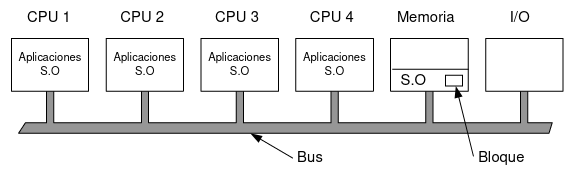
\includegraphics[width=1\textwidth]{resources/multiprocesador_simetrico.png}
                \caption{Representación de multiprocesador simétrico}
                \label{multiprocesador_simetrico}
            \end{figure}
        \end{itemize}

        Podemos clasificarlos también según el modo de ejecución de instrucciones, atendiendo al 
        número de instrucciones y datos que son capaces de procesar a la vez (véase cuadro 
        \ref{modoejecucioninstrucciones}):

        \begin{table}[htp]
            \centering
            \caption{Modos de ejecución de instrucciones}
            \label{modoejecucioninstrucciones}
            \begin{tabular}{rcc}
                \hline
                & \textbf{Un dato} & \textbf{Múltiples datos} \\ \hline
                \textbf{Una instrucción} & SISD & SIMD \\ \hline
                \textbf{Múltiples instrucciones} & MISD & MIMD \\ \hline
            \end{tabular}
        \end{table}

        \begin{itemize}
            \item \textbf{Sistemas SISD} (Single  Instruction  Stream,  Single  Data  Stream). Un 
            procesador procesa secuencialmente instrucciones, y cada instrucción lleva un dato asociado; 
            siendo los sistemas menos efectivos.
            \item \textbf{Sistemas SIMD} (Single  Instruction  Stream,  Multiple  Data  Stream). 
            El procesador ejecuta una instrucción que puede llevar asociada varios datos.
            \item \textbf{Sistemas MISD} (Multiple  Instruction  stream,  Single  Data  stream). Tienen  
            como ventaja fundamental la tolerancia a los fallos. La redundancia de varias unidades de
            proceso trabajando sobre los mismos datos aumenta la fiabilidad del sistema, ya que el fallo 
            de una de las unidades de proceso no supondría ningún inconveniente. Por otro lado, estos 
            sistemas encarecen demasiado la arquitectura y no aumentan el rendimiento ni la velocidad de 
            proceso. 
            \item \textbf{Sistemas MIMD} (Multiple Instruction stream, Multiple Data stream). Este tipo 
            de arquitectura es el más adecuado para una enorme variedad de tareas en las que se desarrollan 
            ejecuciones independientes en paralelo utilizando conjuntos de datos independientes. 

            El procesamiento y ejecución se divide en lo que se llaman hilos, cada uno con su propio 
            procesador, y pertenecientes a uno o varios procesos software. Desde este punto de vista se
            deben controlar bloqueos que se puedan producir por la interferencia de varios hilos a los 
            mismos recursos, como por ejemplo la memoria.

            A nivel de hardware es una arquitectura fácil de implementar, aunque a nivel software se debe
            controlar el acceso compartido con mecanismos como semáforos que eviten los bloqueos mutuos 
            entre procesos. 

            Dentro de esta arquitectura, el procesador y la memoria pueden presentar dos esquemas según 
            estén conectados:
            
            \begin{itemize}
                \item \textbf{Modelos  fuertemente  acoplados}. Los procesadores comparten memoria entre sí,
                lo que puede provocar que en determinadas ocasiones se produzcan bloqueos de acceso.
                Dentro del tipo de acceso a memoria, existen dos tipos:
                
                \begin{itemize}
                    \item \textbf{UMA} o acceso uniforme a memoria.
                    \item \textbf{NUMA} o acceso no uniforme a memoria, donde  la  velocidad  de acceso a 
                    distintas zonas de memoria puede ser distinta.
                \end{itemize}

                Véase figura \ref{modelo_fuertemente_acoplado} para más detalle.
        
                \item \textbf{Modelos   débilmente   acoplados}. Cada procesador gestiona su propia 
                memoria, teniendo como norma el acceso no remoto a memoria (siendo local). Véase figura 
                \ref{modelo_debilmente_acoplado} para más detalle.
            \end{itemize}

            \begin{figure}[!tbp]
                \begin{subfigure}[b]{0.5\textwidth}
                  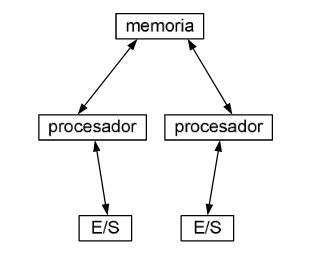
\includegraphics[width=\textwidth, height=\textwidth]{resources/modelo_fuertemente_acoplado_mimd.png}
                  \caption{Modelo fuertemente acoplado}
                  \label{modelo_fuertemente_acoplado}
                \end{subfigure}
                \hfill
                \begin{subfigure}[b]{0.5\textwidth}
                  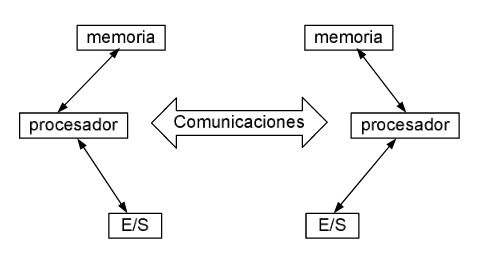
\includegraphics[width=\textwidth, height=\textwidth]{resources/modelo_debilmente_acoplado_mimd.png}
                  \caption{Modelo débilmente acoplado}
                  \label{modelo_debilmente_acoplado}
                \end{subfigure}
                \caption{Modelos de acoplamiento sobre arquitectura MIMD}
              \end{figure}
        \end{itemize}

        \subsubsection{Interconexión de los procesadores}

            El modo en el que los procesadores están conectados es fundamental para el rendimiento
            y velocidad del sistema. Existen diversos modos, pero los cuatro fundamentales son:

            \begin{enumerate}
                \item \textbf{Conexión con bus compartido}. Todos los procesadores están conexionados por el mismo 
                bus, lo que hace que desde el nivel lógico del sistema operativo no sea lo más eficiente, además 
                de dependiente de la velocidad que soporte el propio bus. Véase figura \ref{bus_compartido}.

                \begin{figure}[htp]
                    \centering
                    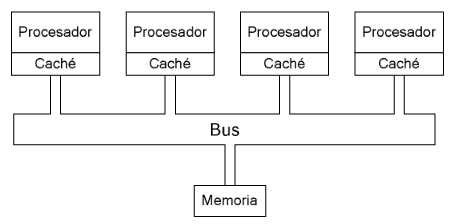
\includegraphics[width=0.7\textwidth]{resources/bus_compartido.png}
                    \caption{Conexión con bus compartido}
                    \label{bus_compartido}
                \end{figure}
    
                \item \textbf{Sistema de barras cruzadas}. Todos los procesadores pueden acceder a todas las 
                memorias simultáneamente, siendo el único retardo la conmutación de barras y haciendo este tipo 
                de conexión más eficiente que la anterior. Aun así, es una arquitectura compleja que necesita 
                $n^2$ conmutadores. Véase figura \ref{barras_cruzadas}.

                \begin{figure}[htp]
                    \centering
                    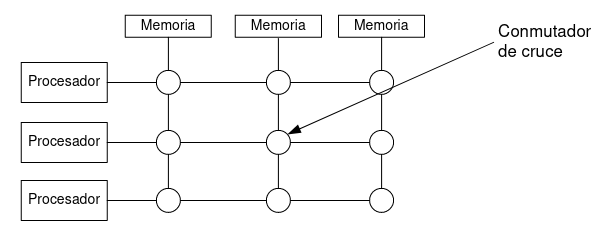
\includegraphics[width=0.8\textwidth]{resources/barras_cruzadas.png}
                    \caption{Conexión con barras cruzadas}
                    \label{barras_cruzadas}
                \end{figure}

                \item \textbf{Conexión mediante hipercubos}. Los procesadores y las memorias se conectan 
                formando hipercubos, siendo la máxima distancia entre nodos $log_2n$ y cada nodo a su vez 
                se conecta con $log_2n$ nodos (cada hipercubo contiene hipercubos de menor dimensión). Esto 
                lo convierte en un modelo complejo pero escalable (complejidad con crecimiento logarítmico, 
                no exponencial). Véase figura \ref{hipercubos}.
                
                \begin{figure}[htp]
                    \centering
                    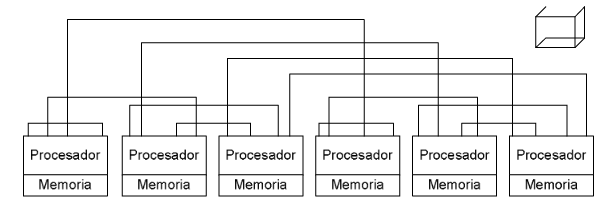
\includegraphics[width=0.8\textwidth]{resources/hipercubos.png}
                    \caption{Conexión mediante hipercubos}
                    \label{hipercubos}
                \end{figure}

                \item \textbf{Conexión mediante conmutadores multietapa}. Está formado por $log_2n$ etapas, 
                donde cada etapa consta de un conjunto de $n$ enlaces conectando a $n/2$ cajas de intercambio.
                Esto lo convierte en un modelo complejo pero escalable (complejidad con crecimiento logarítmico, 
                no exponencial). Véase figura \ref{conmutadores_multietapa}.
                
                \begin{figure}[htp]
                    \centering
                    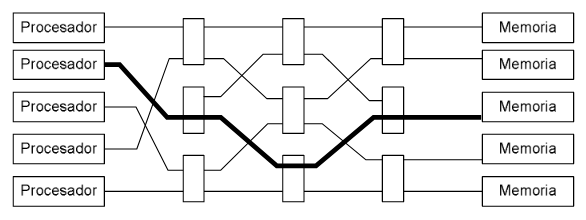
\includegraphics[width=0.8\textwidth]{resources/conmutadores_multietapa.png}
                    \caption{Conexión mediante conmutadores multietapa}
                    \label{conmutadores_multietapa}
                \end{figure}

            \end{enumerate}

    \subsection{Gestión del procesador}

        Para garantizar el correcto funcionamiento de un procesador, se desarrollan operaciones de control y
        gestión. Al existir varios procesadores dentro de una misma máquina, deben actuar y coordinarse como
        un solo procesador virtual.

        \subsubsection{Asignación de los procesadores}

            Dentro de los procesadores del sistema, un procesador puede ser a la vez gestor y trabajador:
            
            \paragraph{Procesador como gestor} Se crea una jerarquía de niveles en la que cada procesador 
            depende de los procesadores situados en un nivel superior. De este modo un procesador recibe 
            órdenes de los procesadores situados en niveles superiores, y asigna trabajos a los 
            procesadores inactivos situados en niveles inferiores. De esta forma se dota al sistma de una 
            mayor tolerancia a fallos.  

            \paragraph{Planificación por oleadas} Un gestor generalmente recibe órdenes que debe repartir 
            a lo largo de la jerarquía. Si puede asignar el trabajo a alguno de los procesadores que están 
            por debajo de él, lo hace, si no trata de ejecutar él el trabajo, y en caso de que no sea 
            posible, lo pasa a niveles superiores. Si llega a la máxima jerarquía y ha sido incapaz de 
            asignarlo, el trabajo se queda en espera pendiente de asignación hasta que haya algún procesador 
            libre.

            \paragraph{Problemas y dificultades} El gestor debe saber cuándo un procesador queda libre de 
            asignación, por lo que debe tener una estimación actualizada de la disponibilidad de cada 
            procesador en cada momento para evitar repartos de carga erróneos.

        \subsubsection{Planificación del procesador}

    \subsection{Sincronización y gestión de la memoria}

        \subsubsection{Algoritmos de sincronización}

% BIBLIOGRAFÍA Y REFERENCIAS
\newpage
\begin{thebibliography}{X}
    \bibitem{} Desarrollo de un sistema expertocon lógica difusa, Jorge Franco Herrera y Angélica Franco Arias \\ \url{https://ingsistycomp.files.wordpress.com/2017/09/proyecto-1-sistema-experto-difuso.pdf}
    \bibitem{} Diseño de un Sistema Experto Difuso para la Determinación de la Densidad de Corriente en una Planta de Cromado, Carolina V. Ponce y Bayron Rojas \\ \url{https://scielo.conicyt.cl/scielo.php?script=sci_arttext&pid=S0718-07642019000200157}
    \bibitem{} Modelo basado en Lógica Difusa para el Diagnóstico Cognitivo del Estudiante \\ \url{https://scielo.conicyt.cl/scielo.php?script=sci_arttext&pid=S0718-50062012000100003}
    \bibitem{} Sistemas Expertos y Lógica Difusa \\ \url{http://catarina.udlap.mx/u_dl_a/tales/documentos/lmt/maza_c_ac/capitulo2.pdf}
    \bibitem{} Sistema de Control Difuso para Unidades de Cuidados Intensivos (UCI), Jefferson Steven Soto Medellín \\ \url{https://repository.ucatolica.edu.co/bitstream/10983/1278/1/Sistemas%20de%20Control%20Difuso%20para%20Unidades%20de%20Cuidado%20Intensivo%20(Trabajo%20Final)%20701429%20Nuevo.pdf}
\end{thebibliography}

\end{document}
